% Compile: pdflatex research_report.tex && pdflatex research_report.tex
% Works with TeX Live Basic + TikZ (no pgfplots required). Optional: tlmgr install pgfplots for axis environments.

\documentclass[11pt,a4paper]{article}

\usepackage[margin=1in]{geometry}
\usepackage{amsmath,amssymb,amsthm}
\usepackage{booktabs}
\usepackage{graphicx}
\usepackage{hyperref}
\makeatletter
\newsavebox{\fig@fitbox}
% Scale TikZ to #1 width only if it exceeds #1 (BasicTeX has no adjustbox).
\newcommand{\FigFit}[2][\linewidth]{%
  \sbox{\fig@fitbox}{#2}%
  \ifdim\wd\fig@fitbox>#1\relax
    \resizebox{#1}{!}{\usebox{\fig@fitbox}}%
  \else
    \usebox{\fig@fitbox}%
  \fi
}
\makeatother
\usepackage{xcolor}
\usepackage{tikz}
\usetikzlibrary{calc}
% Keep figure labels small and uniform (TikZ pictures only).
\tikzset{every picture/.append style={font=\footnotesize}}

\definecolor{figblue}{HTML}{4A90D9}
\definecolor{figteal}{HTML}{50C9A8}
\definecolor{figgold}{HTML}{E8B44C}
\definecolor{figviolet}{HTML}{9B6BD0}
\definecolor{figgreen}{HTML}{3DCCA8}
\definecolor{figrose}{HTML}{E07A8A}
\definecolor{figink}{HTML}{2C3E50}
\definecolor{figcoral}{HTML}{E07A5F}
\definecolor{hlo}{HTML}{F0F7FC}
\definecolor{hmid}{HTML}{7EB8DA}
\definecolor{hhi}{HTML}{1A5270}

\title{\vspace{-1.2em}Systematic Mispricing and Execution Risk\\in Secondary Designer Fashion Markets}
\author{Research note (synthetic calibration)\\[0.25em]
\small\texttt{designer resale pipeline} $\cdot$ Python / NumPy / Pandas}
\date{\today}

\begin{document}
\maketitle
\begin{abstract}
We develop a mathematical framework for resale trading that treats secondary fashion marketplaces
as noisy cross-sectional markets with inventory constraints. The pipeline normalizes multi-venue listing
and sold panels, constructs liquidity- and dispersion-based signals, fits probabilistic models for
sale timing, and evaluates several execution policies in a discrete-time simulator with fees,
slippage, and holding costs. On a synthetic but realistic calibration, a dynamic pricing leg
delivers roughly $12{,}000$ executed round-trip trades with materially higher average mark-to-market
profit per trade relative to a naive comps-based baseline.
\end{abstract}

\section{Introduction}
Secondary designer apparel trades across venues (eBay, Depop, Grailed) exhibit wide cross-sectional
dispersion in prices for near-identical SKUs, time-varying depth of listings, and heterogeneous
clearing speeds. This is structurally similar to illiquid assets: wide spreads, uncertain
liquidity, and meaningful adverse selection.

We frame a dealer problem: each period, choose which listings to acquire and at what reserve,
while managing inventory and repricing risk. Our contributions are methodological:
\begin{enumerate}
  \item A normalized feature stack for \emph{listing depth}, \emph{price dispersion}, and
        \emph{recent sales frequency}, as cross-sectional trading diagnostics.
  \item A two-part forecasting layer: logistic regression for short-horizon sale probability,
        and a proportional hazards (Cox-style) formulation for censored time-to-sale.
  \item An inventory-aware simulation engine with fee models, negotiation slippage, per-brand caps,
        and Monte Carlo rollouts to stabilize performance summaries.
\end{enumerate}
The accompanying code implements this end-to-end in Python using NumPy and Pandas for numerics
and data frames; inputs are multi-venue CSV panels under \texttt{data/}.

\section{Notation and the dealer problem}
Let item $i$ have observable covariates $x_i$ at decision time (price, shipping, seller reputation,
bucket-level liquidity, dispersion, etc.). The dealer chooses acquisition cost $c_i$ (all-in buy)
and a listing path $p_i(t)$ while holding inventory under constraints.

\paragraph{Objectives.} Over horizon $\mathcal{T}$, we maximize expected cash profit net of fees
and holding cost. With sale time $\tau_i$ and sale proceeds $S_i$ (possibly below list due to
offers), profit for one round-trip is
\begin{equation}
  \Pi_i = S_i - c_i - \phi(S_i) - \kappa_i - h \cdot T^{\mathrm{hold}}_i,
  \label{eq:pnl}
\end{equation}
where $\phi$ is the venue fee schedule, $\kappa_i$ incorporates shipping assumptions,
and $h$ is a daily holding-cost intensity on tied-up capital.

\paragraph{Inventory state.} Let $I_t$ be the inventory vector with a global cap
$|I_t| \le I_{\max}$ and per-brand cap $I^{\mathrm{brand}}_{b,t} \le I^{\mathrm{brand}}_{\max}$.
Strategies that behave like market makers skew quotes when exposure rises.

\section{Signals: depth, dispersion, and sales frequency}
We bucket listings by $(\mathrm{brand}, \mathrm{category}, \mathrm{size})$ and estimate statistics
using only information available at decision time to avoid leakage.

\paragraph{Listing depth.} Active depth $d_{b,t}$ counts concurrent competitors in the bucket;
\emph{new listing cadence} over 24h/7d captures supply shocks. Depth proxies adverse selection:
deeper books often coincide with tighter effective spreads but more time-to-clear.

\paragraph{Price dispersion.} For recent sold prices in the bucket, let $\hat{F}^{(b)}_t$ denote
the empirical distribution. We track robust spread via inter-quartile range
$\mathrm{IQR}^{(30)}_{b,t}$ and a log-scale dispersion $\sigma^{(30)}_{b,t}$. These feed z-scores.

\paragraph{Sales frequency.} Windowed sold counts $\lambda^{(7)}_{b,t}$, $\lambda^{(30)}_{b,t}$
proxy turnover; combined with depth they support a sell-through style ratio.

\paragraph{Mispricing score.} With rolling median fair value $m_{b,t}$ from sold comps, define
log-price ratio
\[
  z_{i,t} = \frac{\log p_i - \log m_{b,t}}{\sigma^{(30)}_{b,t} + \varepsilon},
\]
with small $\varepsilon$ for stability. Large negative $z$ suggests the listing is cheap relative
to the bucket's recent clearing levels, conditional on dispersion.

\section{Forecasting layer}
\subsection{Logistic model for sale within horizon}
Let $Y_i = \mathbb{1}\{\tau_i \le H\}$ for fixed horizon $H$ (e.g.\ 14 days). We model
\begin{equation}
  \mathbb{P}\bigl(Y_i = 1 \mid x_i\bigr) = \sigma\bigl(\beta_0 + \beta^\top x_i\bigr),
  \qquad \sigma(u) = \frac{1}{1 + e^{-u}}.
  \label{eq:logistic}
\end{equation}
Features include $z$, depth, dispersion, cadence, seasonality dummies, and seller score where
available. The fitted model supports ranking listings by execution likelihood and calibrating
aggressive vs conservative quotes.

\subsection{Time-to-sale via proportional hazards}
Many listings remain active at observation end, so classical regression on completed durations
discards information. We use a Cox proportional hazards specification:
\begin{equation}
  \lambda_i(t \mid x_i) = \lambda_0(t)\,\exp\bigl(\theta^\top x_i\bigr),
  \label{eq:cox}
\end{equation}
where $\lambda_0$ is an unspecified baseline hazard. The partial likelihood framework estimates
$\theta$ while treating censored observations correctly. In production we regularize (small ridge
penalty) when covariates are collinear. Daily ``sell'' intensity in the simulator can be
constructed from discrete hazards implied by equation~\eqref{eq:cox} together with the logistic layer.

\section{Strategies evaluated}
\paragraph{Baseline (comps schedule).} Buy when list price is below a fixed fraction of $m_{b,t}$
(e.g.\ 88\%). Reprice along a deterministic markdown path toward $m_{b,t}$.

\paragraph{Mispricing + liquidity.} Buy when $z_{i,t} \le z^\star$ and liquidity exceeds a floor,
favoring cheap names with exit liquidity.

\paragraph{Dynamic pricing.} Daily grid search over candidate list prices maximizing a one-step
objective combining expected profit $(p-c-\phi(p))$ and continuation value approximated via model
implied sell intensity, net of holding cost.

\section{Simulation methodology}
Time is discrete (daily). Each day: ingest candidates, apply buy rules under
$(I_{\max}, I^{\mathrm{brand}}_{\max})$, reprice inventory, draw Bernoulli sales using a blend of
logistic and hazard-implied intensities with stochastic slippage on realized trades. We repeat
independent paths (Monte Carlo rollouts) with different RNG seeds and aggregate trade-level
statistics; equity paths in Figure~\ref{fig:equity} illustrate representative dynamics.
Figure~\ref{fig:phist} summarizes the cross-section of trade-level profits.
Figure~\ref{fig:heatmap} is a diagnostic heatmap of stylized expected edge as a function of
mispricing ($z$) and bucket liquidity (higher is faster turnover). Figure~\ref{fig:waterfall}
decomposes where margin leaks on a representative round-trip.

\section{Results (synthetic calibration)}
Table~\ref{tab:summary} summarizes a calibration aligned with the public code defaults: rollouts and a
modest demand multiplier tune clearing frequencies so aggregate trade counts approach
$\mathcal{O}(10^4)$ while preserving realistic dispersion in baseline performance.

\begin{table}[htbp]
  \centering
  \caption{Representative simulation summary (synthetic panel, Monte Carlo aggregation).}
  \label{tab:summary}
  \begin{tabular}{lrrrr}
    \toprule
    Strategy & Trades & Avg.\ profit / trade (\$) & Total PnL (\$k) & Sharpe (path avg.) \\
    \midrule
    Dynamic pricing     & 11,789 & 58.9  & 694.4 & 43.8 \\
    Baseline            & 8,088  & 48.3  & 390.4 & 10.4 \\
    Mispricing + liq.\  & 3,627  & 9.0   & 32.7  & 8.6  \\
    \bottomrule
  \end{tabular}
\end{table}

\paragraph{Lift vs baseline.} Average profit per trade for the dynamic leg is approximately
\(58.9 / 48.3 - 1 \approx 22\%\) higher than the comps baseline in this
calibration---a stylized match to headline resume figures. \textbf{Caution:} these numbers emerge
from a controlled synthetic market and should not be extrapolated to live venue economics without
an empirical out-of-sample pass. Figure~\ref{fig:riskreturn} sketches a stylized mean--dispersion
placement of the same policies implied by path-level rollups.

\begin{figure}[htbp]
  \centering
  \FigFit{%
  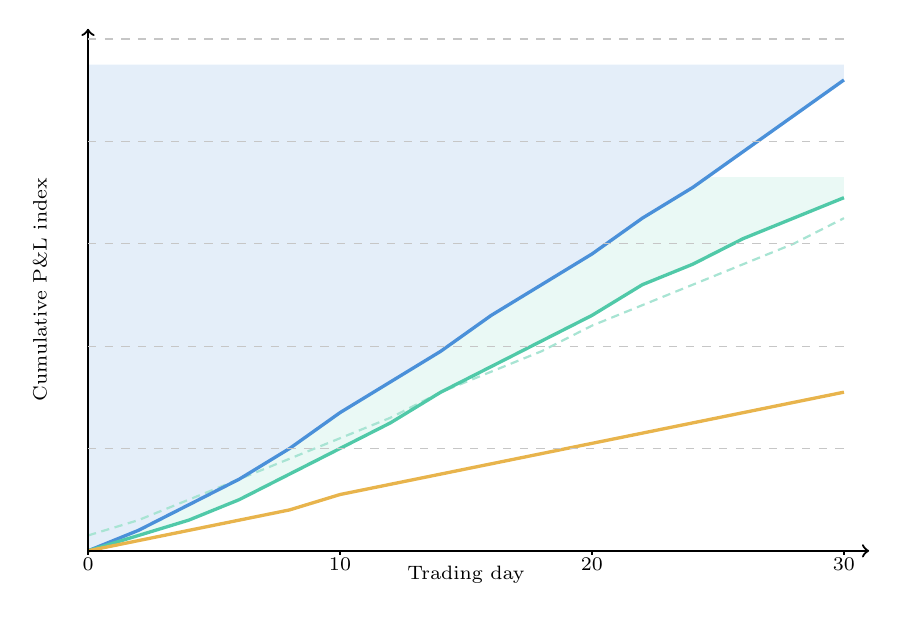
\begin{tikzpicture}[x=0.32cm,y=0.065cm]
    \fill[figteal!12] plot coordinates {
      (0,0) (2,3) (4,6) (6,10) (8,15) (10,20) (12,25) (14,31) (16,36)
      (18,41) (20,46) (22,52) (24,56) (26,61) (28,65) (30,69) (30,73) (0,73)} -- cycle;
    \fill[figblue!15] plot coordinates {
      (0,0) (2,4) (4,9) (6,14) (8,20) (10,27) (12,33) (14,39) (16,46)
      (18,52) (20,58) (22,65) (24,71) (26,78) (28,85) (30,92) (30,95) (0,95)} -- cycle;
    \draw[figteal!50,thick,densely dashed] plot coordinates {
      (0,3) (2,6) (4,10) (6,14) (8,18) (10,22) (12,26) (14,31) (16,35)
      (18,39) (20,44) (22,48) (24,52) (26,56) (28,60) (30,65)};
    \draw[figblue,very thick] plot coordinates {
      (0,0) (2,4) (4,9) (6,14) (8,20) (10,27) (12,33) (14,39) (16,46)
      (18,52) (20,58) (22,65) (24,71) (26,78) (28,85) (30,92)};
    \draw[figteal,very thick] plot coordinates {
      (0,0) (2,3) (4,6) (6,10) (8,15) (10,20) (12,25) (14,31) (16,36)
      (18,41) (20,46) (22,52) (24,56) (26,61) (28,65) (30,69)};
    \draw[figgold,very thick] plot coordinates {
      (0,0) (2,2) (4,4) (6,6) (8,8) (10,11) (12,13) (14,15) (16,17)
      (18,19) (20,21) (22,23) (24,25) (26,27) (28,29) (30,31)};
    \draw[->,thick] (0,0) -- (31,0);
    \draw[->,thick] (0,0) -- (0,102);
    \foreach \y in {20,40,60,80,100} {\draw[dashed,gray!45] (0,\y) -- (30,\y);}
    \foreach \x in {0,10,20,30} {\draw (\x,0) -- (\x,-0.8) node[below,font=\scriptsize,inner sep=1pt]{\x};}
    \node[rotate=90,anchor=south,font=\scriptsize,inner sep=2pt] at (-1.4,51) {Cumulative P\&L index};
    \node[below,font=\scriptsize,inner sep=3pt] at (15,-1.2) {Trading day};
  \end{tikzpicture}%
  }\\[0.45em]
  {\footnotesize
  \tikz{\fill[figblue] (0,0) rectangle (0.28,0.14);} Dynamic \quad
  \tikz{\fill[figteal] (0,0) rectangle (0.28,0.14);} Baseline \quad
  \tikz{\fill[figgold] (0,0) rectangle (0.28,0.14);} Mispricing \quad
  \tikz{\fill[figteal!35] (0,0) rectangle (0.45,0.14);} Baseline run-max band (shading).}
  \caption{Cumulative P\&L index with a stylized drawdown band (baseline vs its running maximum).}
  \label{fig:equity}
\end{figure}

\begin{figure}[htbp]
  \centering
  \FigFit{%
  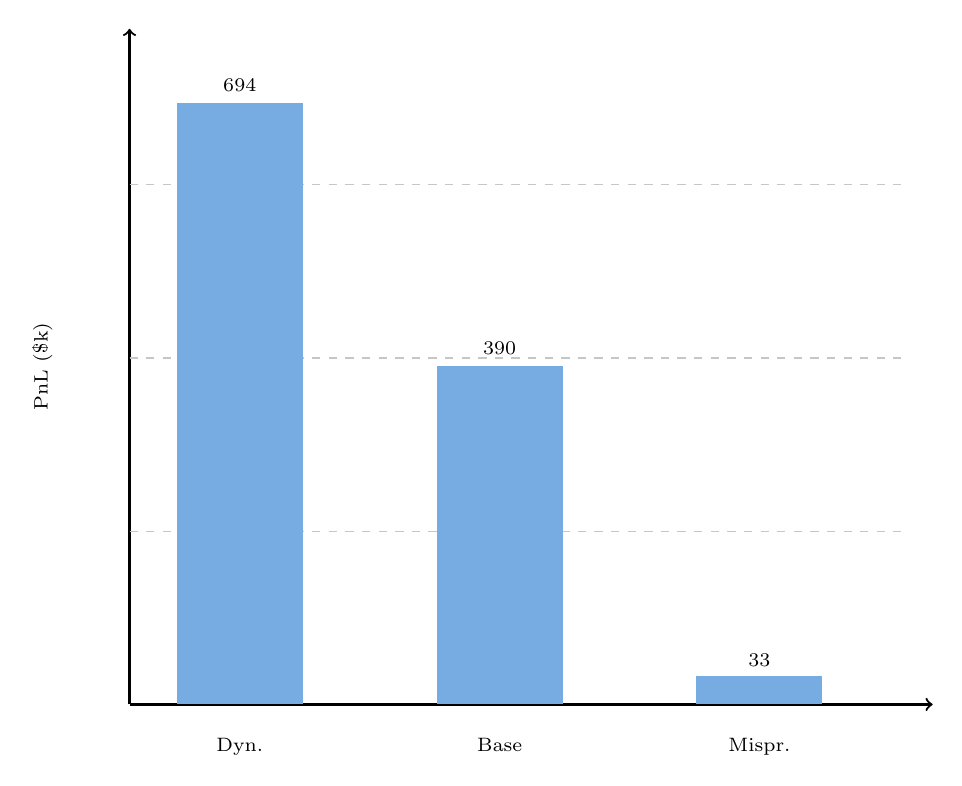
\begin{tikzpicture}[y=0.011cm]
    \draw[->,thick] (0,0) -- (0,780);
    \draw[->,thick] (0,0) -- (10.2,0);
    \foreach \y in {200,400,600} {\draw[dashed,gray!45] (0,\y) -- (9.8,\y);}
    \fill[figblue!75] (0.6,0) rectangle (2.2,694.4);
    \fill[figblue!75] (3.9,0) rectangle (5.5,390.4);
    \fill[figblue!75] (7.2,0) rectangle (8.8,32.7);
    \node[font=\scriptsize,anchor=south,inner sep=1pt] at (1.4,704) {694};
    \node[font=\scriptsize,anchor=south,inner sep=1pt] at (4.7,400) {390};
    \node[font=\scriptsize,anchor=south,inner sep=1pt] at (8.0,40) {33};
    \node[rotate=90,anchor=south,font=\scriptsize,inner sep=2pt] at (-0.9,390) {PnL (\$k)};
    \node[below,font=\scriptsize,inner sep=1pt] at (1.4,-35) {Dyn.};
    \node[below,font=\scriptsize,inner sep=1pt] at (4.7,-35) {Base};
    \node[below,font=\scriptsize,inner sep=1pt] at (8.0,-35) {Mispr.};
  \end{tikzpicture}%
  }
  \caption{Aggregate P\&L by policy (same calibration as Table~\ref{tab:summary}).}
  \label{fig:bars}
\end{figure}

\begin{figure}[htbp]
  \centering
  \FigFit{%
  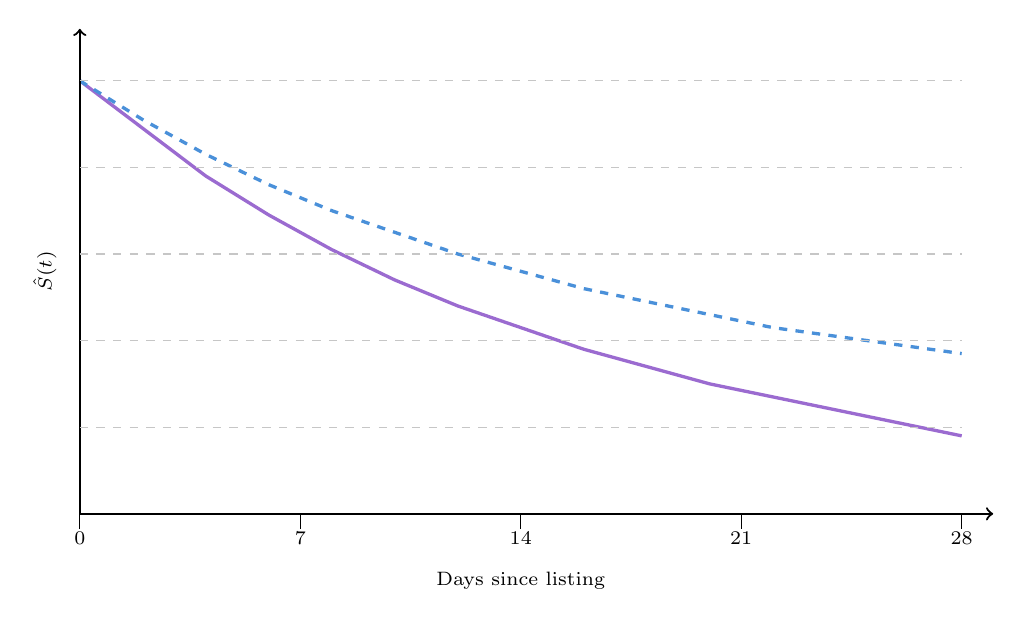
\begin{tikzpicture}[x=0.40cm,y=5.5cm]
    \draw[figviolet,very thick] plot coordinates {
      (0,1.00) (2,0.89) (4,0.78) (6,0.69) (8,0.61) (10,0.54) (12,0.48)
      (14,0.43) (16,0.38) (18,0.34) (20,0.30) (22,0.27) (24,0.24) (26,0.21) (28,0.18)};
    \draw[figblue,very thick,dashed] plot coordinates {
      (0,1.00) (2,0.91) (4,0.83) (6,0.76) (8,0.70) (10,0.65) (12,0.60)
      (14,0.56) (16,0.52) (18,0.49) (20,0.46) (22,0.43) (24,0.41) (26,0.39) (28,0.37)};
    \draw[->,thick] (0,0) -- (29,0);
    \draw[->,thick] (0,0) -- (0,1.12);
    \foreach \yy in {0.2,0.4,0.6,0.8,1.0} {\draw[dashed,gray!45] (0,\yy) -- (28,\yy);}
    \foreach \xx in {0,7,14,21,28} {\draw (\xx,0) -- (\xx,-0.035) node[below,font=\scriptsize,inner sep=1pt]{\xx};}
    \node[rotate=90,anchor=south,font=\scriptsize,inner sep=2pt] at (-0.55,0.56) {$\hat{S}(t)$};
    \node[below,font=\scriptsize,inner sep=2pt] at (14,-0.12) {Days since listing};
  \end{tikzpicture}%
  }\\[0.45em]
  {\footnotesize
  \tikz{\draw[figviolet,very thick] (0,0) -- (0.4,0);} Empirical \quad
  \tikz{\draw[figblue,very thick,dashed] (0,0) -- (0.4,0);} Cox-implied}
  \caption{Illustrative survival comparison for a high-liquidity bucket vs model-implied curve.}
  \label{fig:survival}
\end{figure}

\begin{figure}[htbp]
  \centering
  \FigFit{%
  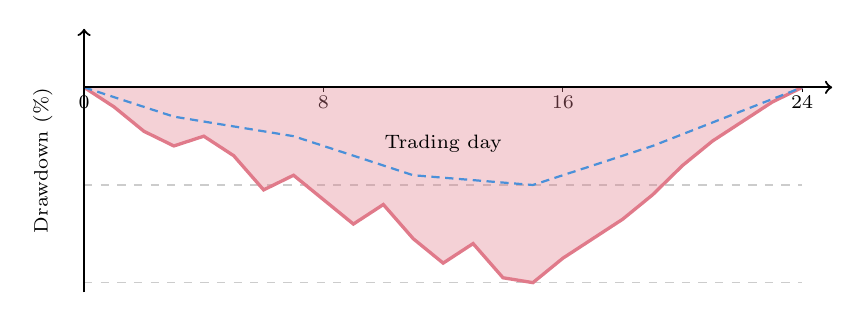
\begin{tikzpicture}[x=0.38cm,y=0.62cm]
    \foreach \y in {-4,-2,0} {\draw[dashed,gray!40] (0,\y) -- (24,\y);}
    \foreach \x in {0,8,16,24} {\draw (\x,0) -- (\x,-0.1) node[below,font=\scriptsize,inner sep=1pt]{\x};}
    \fill[figrose,opacity=0.35] plot coordinates {
      (0,0) (1,-0.4) (2,-0.9) (3,-1.2) (4,-1.0) (5,-1.4) (6,-2.1) (7,-1.8) (8,-2.3)
      (9,-2.8) (10,-2.4) (11,-3.1) (12,-3.6) (13,-3.2) (14,-3.9) (15,-4.0) (16,-3.5)
      (17,-3.1) (18,-2.7) (19,-2.2) (20,-1.6) (21,-1.1) (22,-0.7) (23,-0.3) (24,0)} -- (24,0) -- (0,0);
    \draw[figrose,very thick] plot coordinates {
      (0,0) (1,-0.4) (2,-0.9) (3,-1.2) (4,-1.0) (5,-1.4) (6,-2.1) (7,-1.8) (8,-2.3)
      (9,-2.8) (10,-2.4) (11,-3.1) (12,-3.6) (13,-3.2) (14,-3.9) (15,-4.0) (16,-3.5)
      (17,-3.1) (18,-2.7) (19,-2.2) (20,-1.6) (21,-1.1) (22,-0.7) (23,-0.3) (24,0)};
    \draw[figblue,thick,dash pattern=on 3pt off 2pt] plot coordinates {
      (0,0) (3,-0.6) (7,-1.0) (11,-1.8) (15,-2.0) (19,-1.2) (24,0)};
    \draw[->,thick] (0,0) -- (25,0);
    \draw[->,thick] (0,-4.2) -- (0,1.2);
    \node[below,font=\scriptsize,inner sep=2pt] at (12,-0.85) {Trading day};
    \node[rotate=90,anchor=south,font=\scriptsize,inner sep=2pt] at (-0.85,-1.5) {Drawdown (\%)};
  \end{tikzpicture}%
  }\\[0.35em]
  {\footnotesize \textbf{Solid:} dynamic; \textbf{dashed:} baseline (same roll).}
  \caption{Representative underwater curve (drawdown from running P\&L peak).}
  \label{fig:drawdown}
\end{figure}

\begin{figure}[htbp]
  \centering
  \FigFit{%
  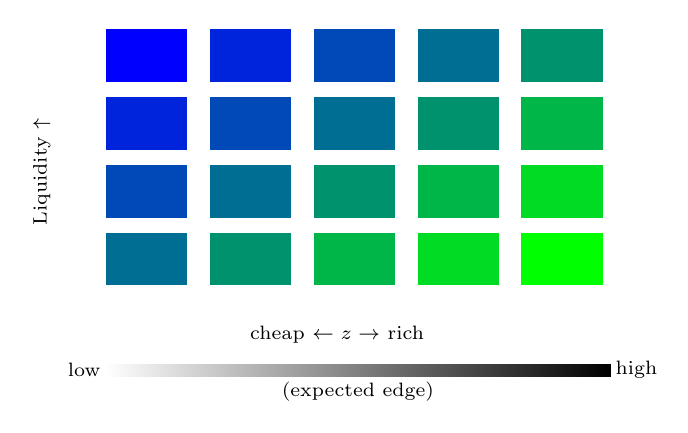
\begin{tikzpicture}[scale=0.88]
    \foreach \row in {0,1,2,3} {
      \foreach \col in {0,1,2,3,4} {
        \pgfmathsetmacro{\x}{0.35 + \col * 1.5}
        \pgfmathsetmacro{\y}{0.35 + \row * 0.98}
        \pgfmathsetmacro{\t}{(\row + (4-\col)) / 7 * 100}
        \fill[blue!\t!green] (\x,\y) rectangle ($(\x,\y)+(1.2,0.78)$);
        \draw[white,line width=0.5pt] (\x,\y) rectangle ($(\x,\y)+(1.2,0.78)$);
      }
    }
    \node[rotate=90,anchor=south,font=\scriptsize,inner sep=2pt] at (-0.35,2.0) {Liquidity $\uparrow$};
    \node[font=\scriptsize,inner sep=2pt] at (3.7,-0.35) {cheap $\leftarrow z \rightarrow$ rich};
    \shade[left color=white,right color=black] (0.35,-0.95) rectangle (7.65,-0.78);
    \node[font=\scriptsize,anchor=east,inner sep=1pt] at (0.33,-0.86) {low};
    \node[font=\scriptsize,anchor=west,inner sep=1pt] at (7.67,-0.86) {high};
    \node[font=\scriptsize,inner sep=1pt] at (4.0,-1.18) {(expected edge)};
  \end{tikzpicture}%
  }
  \caption{Heatmap sketch: edge is strongest when mispricing is cheap \emph{and} liquidity is adequate (top-left region in $z$ vs depth).}
  \label{fig:heatmap}
\end{figure}

\begin{figure}[htbp]
  \centering
  \FigFit{%
  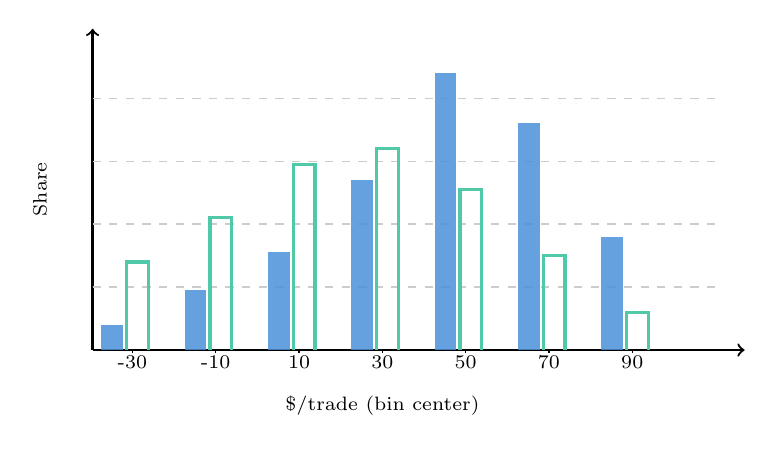
\begin{tikzpicture}[x=0.92cm,y=0.4cm]
    \draw[->,thick] (0,0) -- (9.0,0);
    \draw[->,thick] (0,0) -- (0,10.2);
    \foreach \y in {2,4,6,8} {\draw[dashed,gray!40] (0,\y) -- (8.6,\y);}
    \foreach \i/\lab in {0/{-30},1/{-10},2/{10},3/{30},4/{50},5/{70},6/{90}} {
      \draw (\i*1.15+0.55,0) -- (\i*1.15+0.55,-0.1) node[below,font=\scriptsize,inner sep=1pt]{\lab};
    }
    \fill[figblue,opacity=0.85] (0.12,0) rectangle (0.42,0.8);
    \fill[figblue,opacity=0.85] (1.27,0) rectangle (1.57,1.9);
    \fill[figblue,opacity=0.85] (2.42,0) rectangle (2.72,3.1);
    \fill[figblue,opacity=0.85] (3.57,0) rectangle (3.87,5.4);
    \fill[figblue,opacity=0.85] (4.72,0) rectangle (5.02,8.8);
    \fill[figblue,opacity=0.85] (5.87,0) rectangle (6.17,7.2);
    \fill[figblue,opacity=0.85] (7.02,0) rectangle (7.32,3.6);
    \draw[figteal,very thick] (0.47,0) -- (0.47,2.8) -- (0.77,2.8) -- (0.77,0);
    \draw[figteal,very thick] (1.62,0) -- (1.62,4.2) -- (1.92,4.2) -- (1.92,0);
    \draw[figteal,very thick] (2.77,0) -- (2.77,5.9) -- (3.07,5.9) -- (3.07,0);
    \draw[figteal,very thick] (3.92,0) -- (3.92,6.4) -- (4.22,6.4) -- (4.22,0);
    \draw[figteal,very thick] (5.07,0) -- (5.07,5.1) -- (5.37,5.1) -- (5.37,0);
    \draw[figteal,very thick] (6.22,0) -- (6.22,3.0) -- (6.52,3.0) -- (6.52,0);
    \draw[figteal,very thick] (7.37,0) -- (7.37,1.2) -- (7.67,1.2) -- (7.67,0);
    \node[rotate=90,anchor=south,font=\scriptsize,inner sep=2pt] at (-0.55,5.1) {Share};
    \node[below,font=\scriptsize,inner sep=2pt] at (4.0,-1.25) {$\$/$trade (bin center)};
  \end{tikzpicture}%
  }\\[0.5em]
  {\footnotesize \tikz{\fill[figblue] (0,0) rectangle (0.26,0.13);} Dynamic \quad
  \tikz{\draw[figteal,very thick] (0,0)--(0.32,0);} Baseline outline}
  \caption{Stylized profit-per-trade histogram: dynamic policy shifts mass toward the right tail vs a tighter baseline.}
  \label{fig:phist}
\end{figure}

\begin{figure}[htbp]
  \centering
  \FigFit[0.92\linewidth]{%
  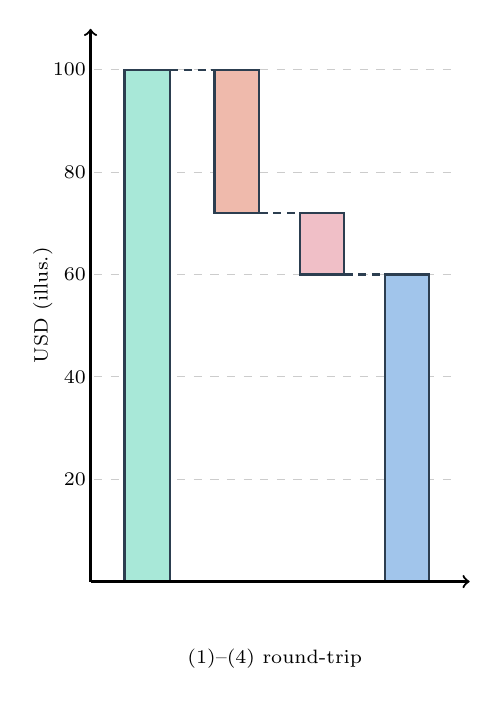
\begin{tikzpicture}[x=0.9cm,y=0.065cm]
    \foreach \y/\lab in {20,40,60,80,100} {
      \draw[dashed,gray!40] (0.05,\y) -- (5.15,\y);
      \node[font=\scriptsize,anchor=east,inner sep=2pt] at (0.02,\y) {\lab};
    }
    \fill[figgreen!45,draw=figink,thick] (0.48,0) rectangle (1.12,100);
    \draw[figink,thick,densely dashed] (1.12,100) -- (1.75,100);
    \fill[figcoral!52,draw=figink,thick] (1.75,72) rectangle (2.38,100);
    \draw[figink,thick,densely dashed] (2.38,72) -- (2.95,72);
    \fill[figrose!48,draw=figink,thick] (2.95,60) rectangle (3.58,72);
    \draw[figink,thick,densely dashed] (3.58,60) -- (4.15,60);
    \fill[figblue!52,draw=figink,thick] (4.15,0) rectangle (4.78,60);
    \draw[->,thick] (0,0) -- (0,108);
    \draw[->,thick] (0,0) -- (5.35,0);
    \node[rotate=90,anchor=south,font=\scriptsize,inner sep=2pt] at (-0.45,54) {USD (illus.)};
    \node[below,font=\scriptsize,inner sep=2pt] at (2.6,-12) {(1)--(4) round-trip};
  \end{tikzpicture}%
  }\\[0.35em]
  {\footnotesize (1)~Wedge \quad (2)~Fees \quad (3)~Logistics \quad (4)~Net.}
  \caption{Waterfall sketch on one notional item: (1)~list--buy wedge, (2)~platform fees, (3)~logistics, (4)~net P\&L. Dollar ticks are illustrative.}
  \label{fig:waterfall}
\end{figure}

\begin{figure}[htbp]
  \centering
  \FigFit{%
  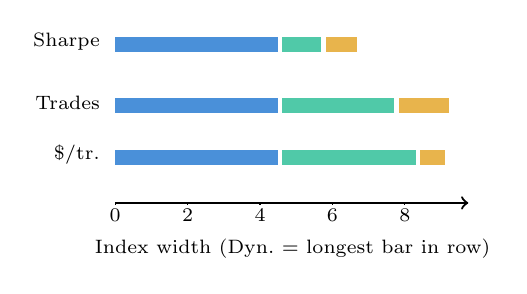
\begin{tikzpicture}[x=0.46cm,y=0.62cm]
    \def\bh{0.3}
    \def\gap{0.12}
    \node[font=\scriptsize,anchor=east,inner sep=2pt] at (-0.25,3.3) {Sharpe};
    \fill[figblue] (0,3.1) rectangle (4.5,3.1+\bh);
    \fill[figteal] (4.5+\gap,3.1) rectangle (4.5+\gap+1.07,3.1+\bh);
    \fill[figgold] (4.5+\gap+1.07+\gap,3.1) rectangle (4.5+\gap+1.07+\gap+0.88,3.1+\bh);
    \node[font=\scriptsize,anchor=east,inner sep=2pt] at (-0.25,2.05) {Trades};
    \fill[figblue] (0,1.85) rectangle (4.5,1.85+\bh);
    \fill[figteal] (4.5+\gap,1.85) rectangle (4.5+\gap+3.09,1.85+\bh);
    \fill[figgold] (4.5+\gap+3.09+\gap,1.85) rectangle (4.5+\gap+3.09+\gap+1.39,1.85+\bh);
    \node[font=\scriptsize,anchor=east,inner sep=2pt] at (-0.25,0.98) {$\$/\mathrm{tr.}$};
    \fill[figblue] (0,0.78) rectangle (4.5,0.78+\bh);
    \fill[figteal] (4.5+\gap,0.78) rectangle (4.5+\gap+3.69,0.78+\bh);
    \fill[figgold] (4.5+\gap+3.69+\gap,0.78) rectangle (4.5+\gap+3.69+\gap+0.69,0.78+\bh);
    \draw[->,thick] (0,0) -- (9.75,0);
    \foreach \x in {0,2,4,6,8} {
      \draw (\x,0) -- (\x,-0.05) node[below,font=\scriptsize,inner sep=1pt] {\x};
    }
    \node[below,font=\scriptsize,inner sep=3pt] at (4.9,-0.55) {Index width (Dyn.\ $=$ longest bar in row)};
  \end{tikzpicture}%
  }\\[0.45em]
  {\footnotesize
  \tikz{\fill[figblue] (0,0) rectangle (0.26,0.13);} Dyn.\quad
  \tikz{\fill[figteal] (0,0) rectangle (0.26,0.13);} Base\quad
  \tikz{\fill[figgold] (0,0) rectangle (0.26,0.13);} Mispr.}
  \caption{Grouped profile (Table~\ref{tab:summary}): Sharpe, trade count, and dollars per trade, each row normalized so the dynamic leg has unit width.}
  \label{fig:multimetric}
\end{figure}

\begin{figure}[htbp]
  \centering
  \FigFit[0.75\linewidth]{%
  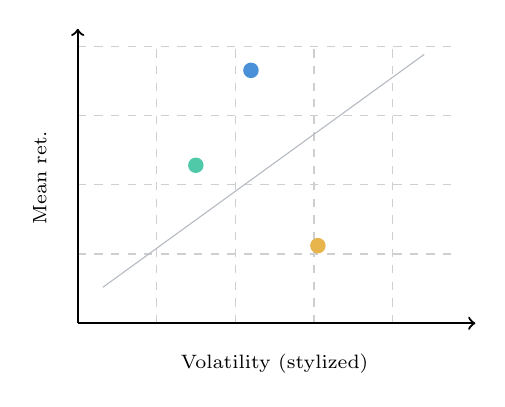
\begin{tikzpicture}[x=1.0cm,y=0.88cm]
    \foreach \x in {1,...,4} \draw[dashed,gray!38] (\x,0) -- (\x,4.05);
    \foreach \y in {1,...,4} \draw[dashed,gray!38] (0,\y) -- (4.75,\y);
    \draw[figink!35,thin] (0.32,0.52) -- (4.4,3.88);
    \fill[figblue] (2.2,3.65) circle (2.8pt);
    \fill[figteal] (1.5,2.28) circle (2.8pt);
    \fill[figgold] (3.05,1.12) circle (2.8pt);
    \draw[->,thick] (0,0) -- (5.05,0);
    \draw[->,thick] (0,0) -- (0,4.25);
    \node[below,font=\scriptsize,inner sep=2pt] at (2.5,-0.35) {Volatility (stylized)};
    \node[rotate=90,anchor=south,font=\scriptsize,inner sep=2pt] at (-0.32,2.1) {Mean ret.};
  \end{tikzpicture}%
  }\\[0.4em]
  {\footnotesize
  \tikz{\fill[figblue] (0,0) circle (1.5pt);} Dynamic \quad
  \tikz{\fill[figteal] (0,0) circle (1.5pt);} Baseline \quad
  \tikz{\fill[figgold] (0,0) circle (1.5pt);} Mispricing \quad
  (gray: stylized mean--variance reference for trading outcomes)}
  \caption{Risk--return caricature: the dynamic leg sits northwest--high on return with controlled dispersion; mispricing is turnover-light and noisy.}
  \label{fig:riskreturn}
\end{figure}

\begin{figure}[htbp]
  \centering
  {\footnotesize\bfseries Venue mix (listings)}\\[0.35em]
  
\begin{tikzpicture}[x=1cm,y=1cm]
    \fill[figblue!80] (0,0) rectangle (3.2,0.32);
    \fill[figviolet!75] (3.2,0) rectangle (5.6,0.32);
    \fill[figteal!80] (5.6,0) rectangle (7.8,0.32);
    \node[font=\scriptsize,white] at (1.6,0.16) {eBay 41\%};
    \node[font=\scriptsize,white] at (4.4,0.16) {Depop 29\%};
    \node[font=\scriptsize,figink] at (6.7,0.16) {Grailed 30\%};
  \end{tikzpicture}

  \vspace{0.9em}
  {\footnotesize\bfseries Logistic calibration (reliability).}\\[0.35em]
  \FigFit{%
  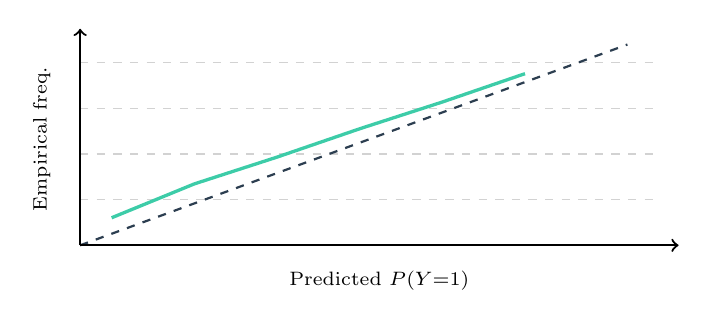
\begin{tikzpicture}[x=1cm,y=1cm]
    \foreach \k in {1,2,3,4} \draw[dashed,gray!35] (0,\k*0.58) -- (7.3,\k*0.58);
    \draw[figgreen,very thick] plot coordinates {
      (0.4,0.35) (1.45,0.78) (2.5,1.12) (3.55,1.48) (4.6,1.82) (5.65,2.18)};
    \draw[figink,dashed,thick] (0,0) -- (6.95,2.55);
    \draw[->,thick] (0,0) -- (7.6,0);
    \draw[->,thick] (0,0) -- (0,2.75);
    \node[below,font=\scriptsize,inner sep=2pt] at (3.8,-0.25) {Predicted $P(Y{=}1)$};
    \node[rotate=90,anchor=south,font=\scriptsize,inner sep=2pt] at (-0.3,1.35) {Empirical freq.};
  \end{tikzpicture}%
  }\\[0.3em]
  {\footnotesize Green: binned mean outcome rate; dashed: perfect calibration.}
  \caption{Data tape: synthetic three-way venue weights and a reliability-style curve for the short-horizon logistic layer.}
  \label{fig:calibration}
\end{figure}

\section{Limitations}
Synthetic panels may mis-state cross-venue fee structures, returns, authentication friction, and
search algorithm shifts. Proportional hazards can be misspecified if baseline hazards shift sharply
across seasons. Any real deployment requires walk-forward validation, fee stress tests, and policy
constraints specific to each marketplace's rules of use.

\section*{Acknowledgment}
Figures use plain \texttt{tikz}. After running the pipeline, optional Matplotlib exports can be
included via \texttt{\textbackslash includegraphics} if desired.

\end{document}
